
\chapter{A Primer for Pybliographer}
\label{cha:rgintro}


This chapter provides an introduction to \Pyb\ for new users.
If you are already familiar with \Pyb, you can skip this chapter.


% Bibliographic database managers are a specialized type of a database
% manager designed for the handling of bibliographic references. They
% are also known as personal information systems, bibliographic
% reference managers, or personal bibliographic software. These systems
% help with three essential research tasks:

%  *  Building a database of references to journal articles, books, and
%     other research publications, using both manual and electronic
%     input methods 
%  *  Searching the created database by author, subject, journal name,
%     and other criteria 
%  *  Generating a list of selected references from
%     the database in a specified format for various purposes

% Options for managing references and other textual information
% -------------------------------------------------------------
%  *   Card based paper index 
%  *   Generic flat file database, e.g., PC File 
%  *   Generic relational database, e.g, MS Access, Paradox, DBase. Some
%      of these will also allow you to include graphics as well as text. 
%  *   Textual database manager. The more generic programs allow one to
%      organize and index text of varying sizes. 
%      AskSam is a leading example of a generic textual database
%      manager. Bibliographic database managers are a
%      customized form of this type of software. See Features of
%      Bibliographic Managers below.  

% Uses of Bibliographic Database Managers
% --------------------------------------------------

%  *   Create course reserve lists and reading lists for students 
%  *   Maintain faculty publication lists 
%  *   Catalog special collections 
%  *   Keep track of reprint collections 
%  *   Maintain bibliographies of references in research areas of
%      personal interest  
%  *   Prepare instantaneous formatted in-text citations and
%      bibliographies during manuscript preparation  
%  *   Create and maintain a reference database shared among a group of
%      resources across a network  
%  *   Publish a web-based bibliography 


\section{How Pybliographer can Help You}
\label{sec:whyuse}




Pybliographer provides Reference manager services to create, load,
modify, list, read, transport, and copy description of resources like
books, articles, and electronic documents, including derivative and
private information.



% [[Many restrictions inherent in the  BibTeX database format used by
% earlier versions of this program are removed or relaxed in this
% version. 

% This version continues to support \BibTeX\ databases to assist you in
% converting to the new database structure. [XXX Subsequent releases,
% however, might not support these features, so we strongly recommend
% conversion to the exclusive use of the new database structure.

% Support for using \BibTeX\ as an import and export format only,
% however, is planned for the foreseeable future.] 
% ]]


To introduce you to the use of \Pyb, we consider three scenarios or
\textit{workflows} first.  Each of these scenarios represents a basic
usage context for the application. In the following they are presented
in sequence of increasing complexity, so that each one is, in fact,
included in the next.



\subsection{Scenario: Search and Browse}
\label{sec:search-browse}

Searching information is certainly the most fundamental (also the most
frequent) task for a reference manager database.  You can look up
records in a variety of ways, starting from whatever information you
have.  There are two ways to start a search, (i) by entering
\textit{search terms}, be it words or \textit{regular expressions}, or
(ii) alternatively by \textit{selecting index terms} from a list.
This list can be a comprehensive index of, e.g., persons taken from
the whole database, or the result of an operation; so you can
effectively follow the associations from article to person to other
article and so on.


\label{sec:workflow1}
In general the searching can be subdivided into the following stages
and tasks:

\begin{table}[htbp]\sffamily\small
  \begin{tabular}[t]{|l|p{10cm}|}
\hline \textbf{Stage}& \textbf{Description}\\ \hline
\textbf{1}& Choose a database, \textit{if necessary}\\
\textbf{2}& Do a \textit{Known-Item-Search}, e.g., with an author\slash
title pair, \textit{or}\\
\textbf{3}& \textit{Browse an Index}, if you are looking for things you
   don't know beforehand (or might have forgotten), e.g., in a Journals
   Index, \textit{or}\\
\textbf{4}& Follow a cross-reference, e.g., by looking at the works of an
   author, or papers which cite another, \textit{or}\\
\textbf{5}& Based on the results, variate or make more precise the search
   question, or even\\
\textbf{6}& Formulate an \textit{expert query}, this requires some
   acquaintance with the data base.\\
\textbf{7}&  \textit{Look over the results.} Examine individual
records. \\
\textbf{8}&  Mark items to set them aside for further examination or
   processing.\\
\textbf{9}& Add a note  to an item.\\
\textbf{10}& Output all or any of the items, in various formats, to another
   file, to the clipboard for inclusion in another document
   (using \textit{Drag-and-drop}), to the printer. \\
\hline
  \end{tabular}
  \label{tab:workflow1}
\end{table}

\newpage

\subsection{Scenario: Write a Paper}
\label{sec:workflow2}

Within the following scenario, you will find yourself searching and
browsing (as above in \ref{sec:search-browse}) many times; now these
\textit{Use Cases} are imbedded in more complex processes. So, e.g.,
stages 6 and 7 below consist not only of searching and browsing
activities, but integrate them with the writing process: an item is
not only found, but it's citation is included in the document in
preparation, it is placed on or taken from a work list, a reference is
linked back to the cited item etc.

\begin{table}[htbp]\sffamily\small
  \begin{tabular}[t]{|l|p{10cm}|}
\hline \textbf{Stage}& \textbf{Description}\\ \hline
&\textbf{Collect Information}\\
\textbf{1}& Maintain a reading list.\\
\textbf{2}& Acquire information from databases.\\
\textbf{3}& Acquire information from other sources.\\
\textbf{4}& Add notes and quotes.\\
& \textbf{Write}\\
\textbf{5}& Maintain a work plan.\\
\textbf{6}& Find items, notes, quotes, etc.\\
\textbf{7}& Insert and mark-up references and quotes.\\
\textbf{8}& Audit work done. (Check cited works, etc.)\\
\textbf{9}& Process references for output formatting.\\
\hline
  \end{tabular}
  \label{tab:workflow1}
\end{table}

\subsection{Scenario: Maintain a Bibliography}
\label{sec:workflow3}

The linking process that lies at the core of \Pyb's support of the
writing process is applied in the next, most demanding situation to
documents of various kinds that are \textit{given} and
\textit{augmented} for better analysis and access.
% Now consider another  situation, where you want to build and maintain
% a website devoted to your favourite writer, A.U.~Thor.   Of course,
% you will want to make maximum use of your computer and derive the
% web presentation from the database. \dots

% A special need is to keep track of things coming in.
% Take reviews, which must be somehow related to the subject work \dots


\begin{table}[htbp]\sffamily\small
  \begin{tabular}[t]{|l|p{10cm}|}
\hline \textbf{Stage}& \textbf{Description}\\ \hline
\textbf{1}& Organise work.\\
\textbf{2}& Add and import records.\\
\textbf{3}& Check, edit and merge records.\\
\textbf{4}& Add documents.\\
\textbf{5}& Describe (mostly) archival items and collections.\\
\textbf{6}& Maintain authority data. \\
\textbf{7}& Add and edit access points.\\
\textbf{8}& Add annotations, other texts.\\
\textbf{9}& Process output.\\
\textbf{10}& Export data for backup, integration.\\
\hline
  \end{tabular}
  \label{tab:workflow1}
\end{table}



% An example scenario follows:

% Let's consider a simple situation first.  During a talk with a friend,
% you suddenly remember a paper that you read a while ago.  Back home,
% you look it up in your Pybliographer Database:

% In the Search Window (Fig. \ref{fig:searchx1}) you enter the author name and
% a word from the title (other approaches are possible and are discussed
% in section XXX):

% \begin{figure}[htbp]
%   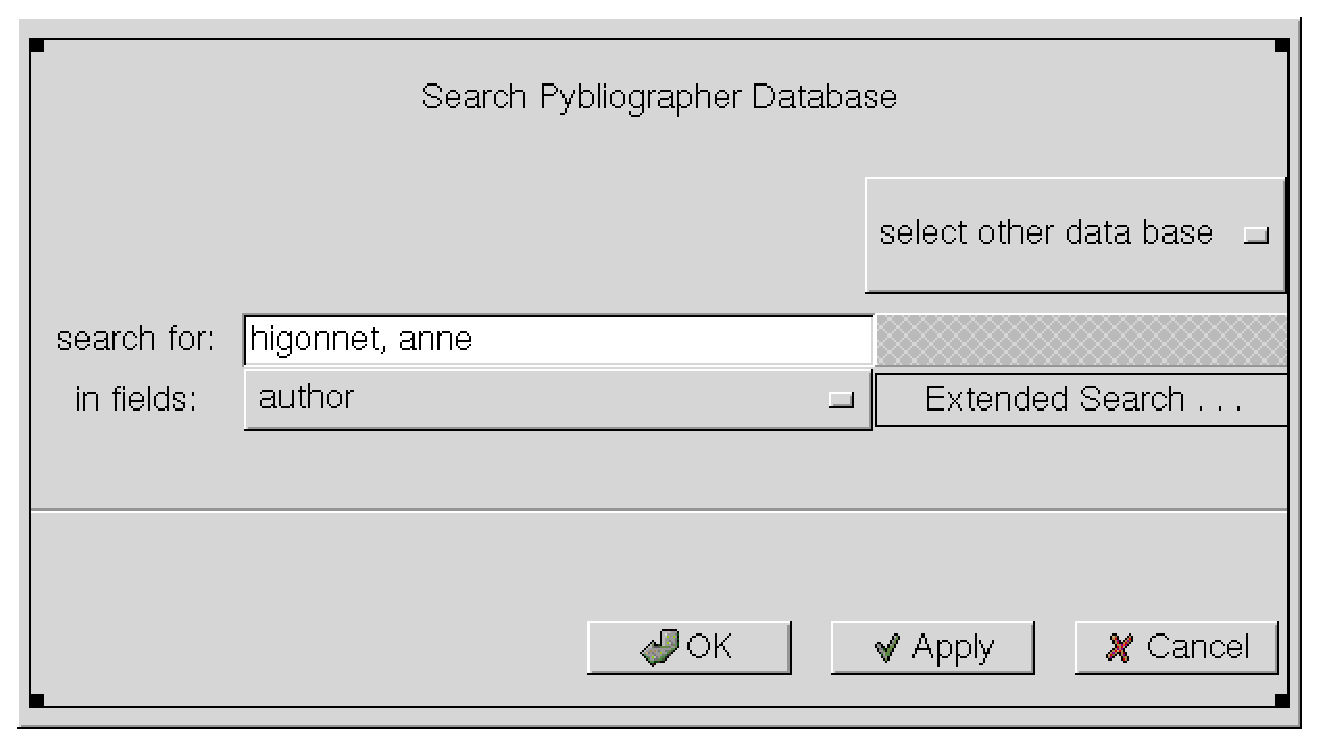
\includegraphics[width=.6\textwidth,bb=0 0 617 342]{pics/searchx1.eps}
%   \caption{Search window with example search terms entered.}
%   \label{fig:searchx1}
% \end{figure}


% The system replies by displaying the list of one item found, and also
% the first and only item in a subwindow (Fig. \ref{fig:searchx2})

% \begin{figure}[h]
  
%   \caption{Display of example search results}
%   \label{fig:searchx2}
% \end{figure}

% You decide to e-mail the citation to your friend. You can easily
% insert it into the e-mail with the standard \textit{drag-and-drop}
% mechanism that Pybliographer supports. The format of the citation is
% easily selected and changed (XXX).

% Perhaps you should try and look for some other references in this area
% when your are in the library again? Let's attach a note to the item,
% so as to be reminded of it when you visit the library the next time: 

% \begin{figure}[ht]
  
%   \caption{Adding an action note}
%   \label{fig:searchx3}
% \end{figure}


% \subsection{Writing an article}
% \label{sec:writing-an-article}

% \label{sec:workflow2}
% \begin{enumerate*}
% \item 
% \end{enumerate*}

% It's only a short note this time, so we don't need much preparation. A
% review say, the book lays on your table, a couple of notes, the editor
% is started. You didn't enter the book into your database yet, so you
% start with querying your national library (see Fig.~\ref{fig:searchx4}
% ). This has the useful side effect of telling you whether the author
% in question has already published something (no need to put your foot
% in it).

% \begin{figure}[ht]
  
%   \caption{Looking up an author in an external database}
%   \label{fig:searchx4}
% \end{figure}

% Whenever you look something up in this way in an \textit{external
%   databaese}, as opposed to the Pybliographer database, the result of
% your query will be captured in an internal list, it is then available
% for further processing, but not yet entered into the Pybliographer
% database. The reason for this is, that it may be too much work for the
% moment -- and it is work that must be done diligently -- to check-in
% and adapt each an every item that a database query might deliver. (See
% the next chapter, in particular ... for more information on this.)
% But in this case, there are but two items, which are easily added.

% If the information comes, as it is here presumably the case, from a
% Z39.50 connected and MARC serving database, there is usually little to
% do at this stage. One point, however, remains to do: the new entries
% must be correctly categorised, lest our fine arrangement goes to
% pieces. If we are content with the standard folder mechanism, it
% should suffice to travers the folder hierarchy until the right leave
% is found, then to drop the item(s).

% \begin{figure}[ht]
  
%   \caption{Dragging an item into a folder}
%   \label{fig:searchx5}
% \end{figure}
 
% To commence the article, you drag the corresponding item on the editor
% window and drop it there: the formatted bibliographical reference is
% inserted and easily edited by you for publication.

% You follow this first paragraph by your observations, occasionally
% consulting your paper notes perhaps. Oh, and this paragraph on page
% 123 you would like to quote, but first you enter it in Pybliographer's
% quotation storage. (XXX) A new editor window appears and already knows
% the item from which you want to enter the text. It first asks you for
% the page number, so you cannot forget it, and then lets you enter and
% edit the text. 

% \begin{figure}[ht]
  
%   \caption{Entering a quotation}
%   \label{fig:searchx6}
% \end{figure}

% By simply dragging the quote into the editor window you not only get
% the text, but the citation as well. You decide to use only a portion
% of the full quote, so you delete a portion of it. Then you want to add
% another voice, whatever was his name \dots\ You decide to open the
% author list and position it at the approximate name.

% \begin{figure}[ht]
  
%   \caption{Displaying the author list}
%   \label{fig:searchx7}
% \end{figure}

% You select and open the right entry (let's assume this), and
% look down the list until you find the wanted entry. From the detail
% view of this entry you could again choose a quote, but then you
% decide otherwise, and simply cite this article instead, you already
% guess, how to do it.

% \begin{figure}[ht]
  
%   \caption{Citing an item}
%   \label{fig:searchx9}
% \end{figure}

% Let's stay for a moment yet with the detil view: the article had been
% quoted, you remember, and selecting the references view lets you find
% this article as well. A sentence from here would fit in much better
% with you review, wouldn't it? 

% \begin{figure}[ht]
  
%   \caption{Excerpt -- sections and quotes}
%   \label{fig:searchxa}
% \end{figure}

% When you are finished with your work, Pybliographer does the
% bibliography for you, simply select Format/references from the
% Menu. You need to specify a stylesheet, and some other options, and
% then you can lay back and relax.

% \begin{figure}[ht]
  
%   \caption{Dialogue Formatting options}
%   \label{fig:dlformat1}
% \end{figure}



% \subsection{Maintaining a Web-Site}
% \label{sec:howwebsite}

\newpage
\section{Bibliographic Records in Pybliographer}
\label{sec:showbibrec}


\begin{dnote}
  \item Show a record display here for entertainment
  \item Explain major UI elements (1 page)
\end{dnote}

%\newpage

%%%%% this table logically pertains to next section

\begin{table}[htbp]\sffamily\small\leftskip-2cm
  \begin{tabular}[t]{|p{8cm}p{8cm}|}
\hline \textbf{Description}& \textbf{Examples} \\
\hline
\textbf{Bibliographical Description}\par
 According to ISBD, this comprises the title and statement of
 resposibility area, the edition area, the materials specific area, the
 publication statement area, the physical description area, the series
 statement area, the notes area, and the standard numbers and terms of
 availibility area.
 &
 {\obeylines
 +Der+ Zauberberg / Thomas Mann
 A l'ombre des jeunes filles en fleurs / Marcel Proust
 [kit] [motion picture] [art original] 
 31. Aufl. \quad In full score 
 Vol. 1, no. 1 (winter 1957)-
 Scale 1:3,500,000
 Amsterdam: N. Israel, 1973
 vi, 754 p. : ill. (some col.); 24 cm
 (Actualit\'es scientifiques et industriels; 1236)
 Thesis (Ph.D.) -- University of Michigan, 1971
 Includes Indexes
 }\\
\textbf{Access Points}\par
This is information that characterises the item in terms which are,
generally speaking, not taken from the item, at least not verbatim.
Using a controlled vocabulary is als known as authority control, lists
of such terms are called authority files.\par
Names of persons and corporate bodies are (for the orthodoxy) the most 
important access points, and pose characteristic problems. Other types
of data in this class are subject headings, classifications, keywords
and uniform titles.
&{\obeylines
Albertus <Magnus>
Montherlant, Henry +de+ 
Alvarez Quintero, Seraf\'in, 1871-1938
Paulus <Apostolus>: Epistolae ad Thessalonicenses
Deutscher Biologentag <6, 1964, Hersfeld>
Programming languages (Electronic computers)
30 A 58 \quad D.3 \quad 11103-57-4 (Vitamin A)
EC 4.1.3.1 (isocitrate lyase) 
}\\
\textbf{Contents related information}\par
This includes all information taken from the item at hand, be it
transcribed verbatim or not.
&
{\obeylines
Abstract
Short summary note
Quotation
Excerpt
ad-hoc keyword
}\\
\textbf{Task related data}\par
This information is used to keep track of various tasks associated
with the reading and using of resources. 
&{\obeylines
Project/reading list
Desiderata
Orders (bookseller, inter-library loan)
Items by location (library, shelf)
}\\
\textbf{Holdings information}\par
Information that is neccessary to gain access to an item
&
{\obeylines
URL \quad file name 
Call number \quad Shelf number 
Institution (library) code
Shelving place, binder (for copies)
}\\
\hline
    \end{tabular}
  \caption{Information stored in a reference manager}
  \label{tab:knorrtyp}
\end{table}
\newpage
\section{Describing Resources}
\label{sec:introdesc}
\nopagebreak
\begin{dnote}
  \item Give an overview of the requirements for various user
    situations (cf. Eversberg, ...)
  \item Introduce to the Chapter 3 treatment of planning decisions
    w.r.t. level of description, use of classifications, \textit{rigeur}
  \item Background for daily work, giving overall direction. 
\end{dnote}
Before we can search for them, the resources of interest must be
identified and described. \dots 
\begin{itemize*}
\item To identify
\item To distinguish
\item To access
\end{itemize*}





\subsection{A Model of Bibliographical Data}
\label{sec:introdata}

A model of the data that is relevant for our application (taken from
Knorr \citep{knorr98}) is shown in Table \ref{tab:knorrtyp} on page
\pageref{tab:knorrtyp}.


% \label{sec:introacc}

% Not infrequently we might want to a little reading. \Pyb\ can help us
% here in many ways:
% \begin{itemize*}
% \item By searching for a title -- looking for holdings information
% \item By providing on-line access
% \item By helping organise our work
% \end{itemize*}




% \section{General considerations}
% \label{sec:descgen}


% When describing ressources of any kind, we encounter some problems
% again and again. 

% The first has to do with the question which information to use; more
% specifically where to look for the information.

% To reduce the variation and confusion when describing ressources, there
% are certain established principles, among others:

% \begin{itemize}
  
% \item Use the original text, if possible. This principle avoids e.g.,
%   the confusion arising from giving a place of publication that is
%   \textit{K�ln, C�ln, Keulen, Cologne}, depending upon time and place
%   of cataloguing. 
% \item Use special normalised forms to account for the needs of users
%   that might not know the original form, but do not replace the
%   original form (for important pieces of information), but give both
%   of them.
% \item Prefer the information as it is found on the title page (and
%   some comparable places).  At least indicate information that does
%   not come from the standard places by putting it into brackets [].
% \item Distinguish the various classes of information, in particular do
%   not confound formal and material description, nor bibliogrpahic
%   description and annotations etc. although the software supports it
%   both. It much simplifies life to keep these purposes apart.
% \end{itemize}


\section{Exploiting [Working with] Resources}
\label{sec:introexpl}

We do not acquire, store, and browse bibliographical records for their
own sake, but in order to put them to use.  For at least as long as we
are sitting at our thesis it is our daily task to use them and we
want to make the most of them, and of the fatures that  \Pyb\ offers.

The most basic use is, of course, citing a source. Often that includes
taking a quote from it. Then we might want to obtain a list of cited
works (references), but also need support for our work in form of list
of references eyemarked, or already used, or yet to be considered. It
is furthermore helpful to be able to flexibly handle quotations.\dots

Often our memory is not quite up to the task and we want assistance in 
using sources, tha \Pyb\ happily provides. It allows us to store
quotes, to add notes, even longer excerpts and reviews, if we want. We
can not only cite them comfortably, but also search them without
regard to their being stored within or out of the database proper. 

Finally, if our work continues for a while, we may find the many ways
useful, that \Pyb\ provides to \textit{organise} the database. So we
can ask for \textit{subjects} by means of attaching subject headings
or classification codes, we can trace editions and reviews of or
references to a work, and we can keep track of our own work.


\section{Special Materials}
\label{sec:introsmd}


Many reference managers are geared towards the formatting of
references most frequent in scientific\slash technical papers, almost
as much as library type applications are towards the cataloguing of
monographs.

In contrast \Pyb\ tries to be adaptable and extensible enough to
support the specialist, while not losing its usability for the average
user (which the specialist remains to be, after all, outside of his
area of specialisation).

What does that mean? \Pyb\ provides an extensible, open, and adaptable
database schema, and appliction programming interface (API).  More
about extending and adapting \Pyb\ can be found in chapter
\ref{cha:pscript}.  An interface alone, however is not sufficient. 
Of equal or possibly even greater importance is a sound database
structure, something missing from most popular alternatives. More
about the database structure you can find in section \ref{sec:rgccont}.

In the following a number of specific requirements are detailed,
together with an indication of what \Pyb\ does offer you in that
respect.

\begin{description}
\item[Archival and administrative records] need a different treatment
  because they are unique, depending on context (provenance) for
  description, access, and interpretation.  Thus they require a
  multi-level description, as item but also on the collection level.
  In addition, they often form series, that warrant structured
  annotations for analysis, \dots
\item[Continuing resources, collections] include serials, journals,
  web-sites, e-journals, and the like (user-maintained, so-called
  artificial collections are similar enough to warrant mention here).
  The degree of \textit{description} that is usually needed varies
  considerably, what is important, however, is the support \Pyb\
  provides for not-so frequent situations.
\item[Multi-level description] is generally available and helps with
  handling of articles in journals (journal data are stored and
  maintained separately) monographs in series, documents on web-sites, 
 and so on.
\item[Analytical annotations] add to the annotation facilities with
  the option of form-based or tabular data entry.  Typical situations
  are preparation of meta-analyses or historical case
  analyses. (Example \dots) (This is really a requirements statement
  XXX)
\item[Music] is supported by (i) multilevel description for, e.g.,
  sound recordings, where more than one piece is on one carrier, and
  (ii) by handling \textit{works}, allowing searching and displaying
  of multiple recordings but also manuscript or printed scores,
  etc. 
\item[Audio and Video Recordings] and many other materials can be
  correctly described  
\end{description}

\begin{dnote}
\item This section should alert the user to the fact that the needs of
  particular kinds of materials are looked after, -- and that there
  are such special needs.
\item I would rather like a table: Material -- Problem -- Solution
\item Cf. AACR2R for a list of special materials (and \textsf{MARC 007})
\end{dnote}

\section{Special Needs}
\label{sec:introspecial}

\begin{dnote}
  \item More processing related questions?
\end{dnote}



%%% Local Variables: 
%%% mode: latex
%%% TeX-master: "UG"
%%% End: 
